% !Mode:: "TeX:UTF-8"
% VL 8, gebaut aus part-representation-learning/14-autoencoder.md
% (Dialogmuster: transcripts/vl07-netze-von-hand-autoencoder-2025 und
%  transcripts/vl08-vae-word2vec-2025/notiz.md, Abschnitt Autoencoder-Varianten).
% !Mode:: "TeX:UTF-8"
\newcommand{\thepage}{} % to silence a hyperref warning about pdfpagelabels
\RequirePackage[]{silence}
\WarningsOff[hyperref]
\PassOptionsToPackage{log-declarations=false}{xparse}
%\RequirePackage[l2tabu, orthodox]{nag}
\RequirePackage{luatex85} % to make \pdf...= commands work with LuaTeX
\documentclass[aspectratio=169,t]{beamer}
\usepackage{ifthen}
\usepackage[T1]{fontenc}
\usepackage{iftex}
\ifLuaTeX
 \usepackage{fontspec}
 \setmainfont[Ligatures=TeX]{Source Sans Pro}
\else
 \usepackage[utf8]{inputenc}
\fi
\usepackage{german}
\usepackage{newunicodechar}
\newunicodechar{€}{\texteuro}
\newunicodechar{ß}{\ss}
\renewcommand{\SS}{\iffontchar\font"1E9E \symbol{"1E9E}\else SS\fi}
\usepackage{ellipsis}
\usepackage{microtype}
\usepackage{listings}
\usepackage{sourcecodepro}
\lstset{language=Python, basicstyle=\ttfamily}
\usepackage{amsfonts}
\usepackage{amssymb}
\usepackage{amsthm}
\usepackage{fancyhdr}
\usepackage{graphicx}

\newtheorem{proposition}[theorem]{Proposition}

\DeclareMathOperator*{\argmax}{argmax}
\DeclareMathOperator{\supp}{supp}
\newcommand{\E}{\ensuremath{\mathbb{E}}}
\newcommand{\V}{\ensuremath{\mathbb{V}}}

\setbeamercolor{emph}{fg=purple}
\renewcommand<>{\emph}[1]{%
  {\usebeamercolor[fg]{emph}\only#2{\itshape}#1}%
}



\hypersetup{draft=false,colorlinks=false,pdfpagemode=UseOutlines,plainpages=false,
            breaklinks=true,bookmarksnumbered=true,pdfborder=0 0 0,
            pdftitle={Einführung in Deep Learning WiSe 2026/27 HHU},
            pdfauthor={Konrad Voelkel},
            pdfsubject={data science}}

%\documentclass[aspectratio=169,t]{beamer}
\usetheme{hhubeamer} % put the hhu-beamer-theme in /usr/share/texmf/tex/latex/beamer/themes/

% -------------------- Code listings config --------------------
% Define custom colors for syntax highlighting
\definecolor{codegreen}{rgb}{0,0.6,0}
\definecolor{codegray}{rgb}{0.5,0.5,0.5}
\definecolor{codepurple}{rgb}{0.58,0,0.82}
\definecolor{backcolour}{rgb}{0.96,0.96,0.94} % Very light gray/beige
% Configure the listings package
\lstset{
    language=Python,
    backgroundcolor=\color{backcolour},   
    commentstyle=\color{codegreen}\itshape,
    keywordstyle=\color{blue}\bfseries,
    numberstyle=\tiny\color{codegray},
    stringstyle=\color{codepurple},
    basicstyle=\ttfamily\footnotesize, % Use a monospaced font
    breakatwhitespace=false,         
    breaklines=true,      
             % Enable automatic line breaking
    captionpos=b,                      % Caption at the bottom
    keepspaces=true,                 
    numbers=left,                      % Line numbers on the left
    numbersep=10pt,                    % Distance of line numbers from the code
    showspaces=false,                
    showstringspaces=false,            % Don't show weird underscores in strings
    showtabs=false,                  
    tabsize=4,
    frame=single,                      % Add a subtle border around the code
    rulecolor=\color{black!20},        % Border color
  }

\event[]{}
\author[Wintersemester 2026/27]{Dr. Konrad Völkel, Wintersemester 2026/27}

%\title{Data Science, VL 1}
%\date{16.04.2026}


%%% Local Variables:
%%% mode: latex
%%% TeX-master: t
%%% End:


% Fassung mit Dozentennotizen (zweiter Schirm): die nächste Zeile einkommentieren.
% \setbeameroption{show notes on second screen=right}

\graphicspath{{../images/}}

\title[Autoencoder (VL 8)]{Autoencoder\\\large Einführung in Deep Learning, VL 8}
\date{02.12.2026}

\begin{document}

\begin{frame}
  \titlepage

  \note{\textbf{Ablauf, 90 Minuten.} 2025 verteilt auf das Ende von VL 7 und den Anfang
    von VL 8 (dort 33 Min. für die Varianten):\\[2pt]
    \begin{tabular}{@{}rll@{}}
      0--10  & Folien 2--4   & Lernen ohne Label, die Idee\\
      10--20 & Folien 5--6   & Loss, Schema, Vergleich mit PCA\\
      20--30 & Folien 7--8   & MNIST, das Layout\\
      30--45 & Folien 9--10  & \textbf{Code: Architektur und Training}\\
      45--55 & Folie 11      & Tricks beim Training\\
      55--65 & Folien 12--13 & Label Autoencoder, zwei Köpfe\\
      65--75 & Folie 14      & Architektur-Tricks: Dropout, BatchNorm\\
      75--88 & Folien 15--17 & Sparse und Denoising\\
      88--90 & Folie 18      & Blatt 8\\
    \end{tabular}\\[4pt]
    Der Autoencoder ist das erste Modell, das nicht klassifiziert --- den Perspektivwechsel
    („die Label sind die Eingaben selbst“) langsam machen.}
\end{frame}

\begin{frame}
  \frametitle{Was, wenn wir keine Label haben?}

  \begin{center}
    \Large
    Bisher: $y = f(x)$ schätzen, mit bekannten $y$.\\[16pt]
    Jetzt: keine $y$. Wie misst man dann Erfolg?
  \end{center}

  \note{Die Frage in den Raum stellen und sammeln lassen. Das ist der Perspektivwechsel
    der Sitzung, und er lohnt drei Minuten Stille.}
\end{frame}

\begin{frame}
  \frametitle{Die Idee}

  \begin{center}
    \Large
    $f$ unbekannt --- aber $g(f(x)) = x$ bekannt.\\[16pt]
    \normalsize $f$ = Encoder, \quad $g$ = Decoder
  \end{center}

  \note{Ziel: die Eingabe in ein anderes Koordinatensystem transformieren und wieder
    zurück --- und messen, wie gut das klappt.
    Sofortiger Einwand, den man selbst bringen sollte, wenn er nicht kommt: Das ist
    trivial, nimm $f = g = \operatorname{id}$.}
\end{frame}

\begin{frame}
  \frametitle{Die Einschränkung macht es interessant}

  \begin{center}
    \Huge $f \colon \mathbb{R}^n \to \mathbb{R}^k$, \quad $k \ll n$
  \end{center}

  \bigskip
  \begin{center}
    \normalsize Der Encoder muss lernen, was \emph{wesentlich} ist.
  \end{center}

  \note{Dimensionsreduktion ohne Informationsverlust --- das ist der Flaschenhals.
    Wer Data Science gehört hat, denkt an PCA. Der Vergleich kommt gleich.}
\end{frame}

\begin{frame}
  \frametitle{Loss und Schema}

  \begin{center}
    \Large $L(x; f,g) = \frac1N \sum_i \| x_i - g(f(x_i))\|^2$
  \end{center}

  \begin{center}
    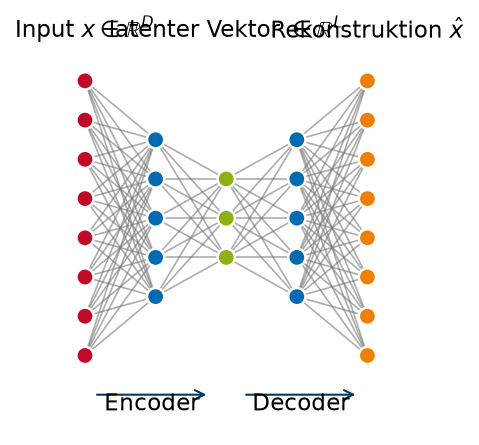
\includegraphics[height=0.42\textheight]{vl06-autoencoder-schema.png}
  \end{center}

  \note{MSE zwischen Ein- und Ausgabe, die Label sind die Eingaben selbst ---
    \emph{self-supervised}.
    Nebenbemerkung, die 2025 gut ankam: Der Autoencoder ist eigentlich gar kein Deep
    Learning im engeren Sinn, die Idee ist viel älter.}
\end{frame}

\begin{frame}
  \frametitle{Autoencoder gegen PCA}

  \begin{center}
    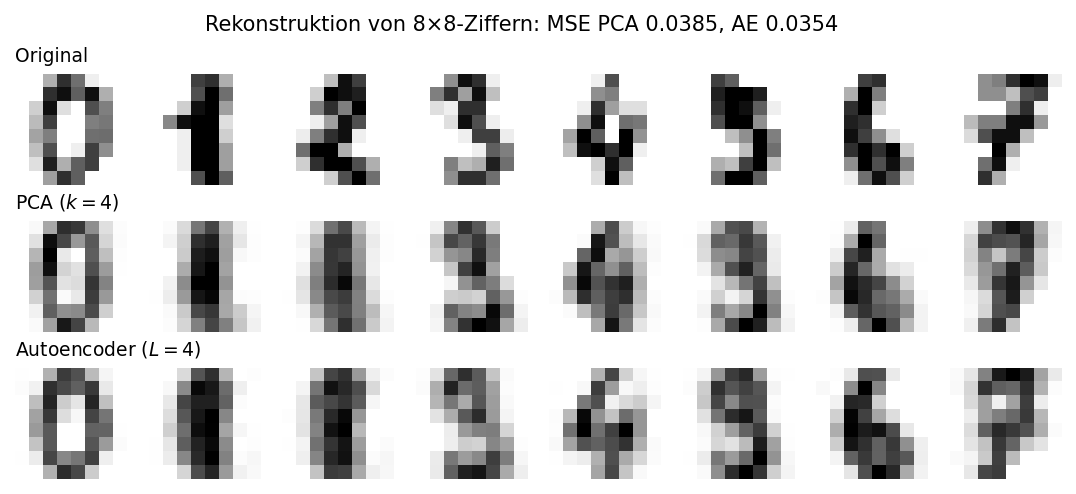
\includegraphics[width=0.72\textwidth]{vl06-ae-vs-pca.png}
  \end{center}

  \note{Ein \emph{linearer} Autoencoder findet denselben Unterraum wie PCA. Mit
    Nichtlinearitäten erfasst er gekrümmte Strukturen, die PCA verfehlt --- bei gleicher
    Dimension des Flaschenhalses deutlich bessere Rekonstruktion.
    Das ist das Argument, warum sich der Aufwand lohnt.}
\end{frame}

\begin{frame}
  \frametitle{MNIST}

  \begin{center}
    \Large
    $28 \times 28$ Graustufen, Ziffern 0--9\\[8pt]
    60\,000 Training, 10\,000 Test
  \end{center}

  \bigskip
  \begin{center}
    \normalsize
    Kompression \quad Generieren \quad Klassifikation
  \end{center}

  \note{Vier Tasks auf denselben Daten: unsupervised komprimieren; unsupervised neue
    Bilder erzeugen (nächste Woche, VAE); supervised klassifizieren; supervised Bilder
    mit vorgegebener Ziffer erzeugen.
    Heute die ersten beiden Spalten: Kompression und Klassifikation.}
\end{frame}

\begin{frame}
  \frametitle{Das Layout}

  \begin{center}
    \Large
    Encoder: $D \to L$ \qquad Decoder: $L \to D$\\[16pt]
    \normalsize Datenraum (Pixel) --- latenter Raum --- Datenraum
  \end{center}

  \note{Der Begriff \emph{latenter Raum} fällt hier zum ersten Mal richtig und trägt den
    Rest des Semesters. Bei Bildern heißt der Datenraum Pixelraum.}
\end{frame}

\begin{frame}[fragile]
  \frametitle{Code: die Architektur}

  \lstset{basicstyle=\ttfamily\scriptsize}
  \begin{lstlisting}
class Autoencoder(nn.Module):
    def __init__(self, latent_dim=12):
        super().__init__()
        self.encoder = nn.Sequential(
            nn.Linear(IMAGESIZE**2, 256), nn.ReLU(True),
            nn.Linear(256, 64), nn.ReLU(True),
            nn.Linear(64, latent_dim))
        self.decoder = nn.Sequential(
            nn.Linear(latent_dim, 64), nn.ReLU(True),
            nn.Linear(64, 256), nn.ReLU(True),
            nn.Linear(256, IMAGESIZE**2), nn.Sigmoid())

    def forward(self, x):
        latent = self.encoder(x)
        return latent, self.decoder(latent)
  \end{lstlisting}

  \note{Zwei \texttt{nn.Sequential}-Blöcke, symmetrisch. Das Sigmoid am Ende des Decoders
    sorgt dafür, dass die Ausgabe wie Pixelwerte in $[0,1]$ liegt.
    Frage, die kommen wird: Warum am Encoder kein Sigmoid? Antwort: nötig erst beim
    Sparse Autoencoder, dessen Strafterm latente Werte in $[0,1]$ voraussetzt. Man
    \emph{kann} es setzen.
    \texttt{forward} gibt beides zurück --- den latenten Vektor braucht man später.}
\end{frame}

\begin{frame}[fragile]
  \frametitle{Code: das Training}

  \lstset{basicstyle=\ttfamily\scriptsize}
  \begin{lstlisting}
data_loader = DataLoader(mnist_data, batch_size=512, shuffle=True)
optimizer = optim.SGD(model.parameters(), lr=1e-2)

for epoch in range(15):
    for img, labels in data_loader:
        latent, reconstructed = model(img)
        loss = reconstruction_criterion(reconstructed, img)
        optimizer.zero_grad(); loss.backward(); optimizer.step()
  \end{lstlisting}

  \note{Neu gegenüber VL 3 sind \texttt{Dataset} und \texttt{DataLoader}: Der Datensatz
    liefert einzelne Samples (mit einer \texttt{transform}, die das Bild zu einem Vektor
    der Länge 784 macht), der Loader mischt und bündelt zu Mini-Batches.
    Die Schleife selbst ist dieselbe wie immer --- nur dass das Label das Bild ist.
    \textbf{Ehrlich sein:} Mit diesen Werten (SGD, \texttt{lr=1e-2}, 15 Epochen) sinkt der
    MSE nur von 0,231 auf 0,228 --- man sieht Matsch. Das ist Absicht und die Überleitung
    zur nächsten Folie. Zum Vergleich gemessen: Adam mit \texttt{lr=1e-3} kommt auf 0,019.}
\end{frame}

\begin{frame}
  \frametitle{Tricks beim Training}

  \begin{itemize}\setlength{\itemsep}{6pt}
  \item Mehr Epochen --- aber Early Stopping
  \item Data Augmentation
  \item Lernrate anpassen
  \item Weight Decay ($L^2$-Regularisierung)
  \item \emph{Adam statt SGD}
  \end{itemize}

  \note{Die Liste räumt auf, was die vorige Folie angerichtet hat. Faustregel für den Rest
    des Kurses: Adam statt SGD, ohne dass wir Optimierer vertiefen --- was Adam tut, steht
    im Kapitel „Optimierer“.
    Early Stopping: aufhören, wenn der Testloss wieder steigt, während der Trainingsloss
    weiter sinkt.}
\end{frame}

\begin{frame}
  \frametitle{Supervised: Klassifikator aus dem Encoder}

  \begin{center}
    \Large
    Encoder $\to$ Linear auf 10 $\to$ Softmax
  \end{center}

  \bigskip
  \begin{center}
    \normalsize Loss: Kreuzentropie (\texttt{nn.CrossEntropyLoss} auf den Logits)
  \end{center}

  \note{Kreuzentropie $=$ negative Log-Likelihood $\mathrel{\hat=}$ KL-Divergenz zwischen
    echten Labels und Vorhersage --- das war Blatt 5.
    \texttt{CrossEntropyLoss} macht Softmax und NLL in einem Schritt, numerisch stabil
    (VL 4!) --- deshalb bekommt es die Logits, nicht die Wahrscheinlichkeiten.}
\end{frame}

\begin{frame}
  \frametitle{Warum nicht beides?}

  \begin{center}
    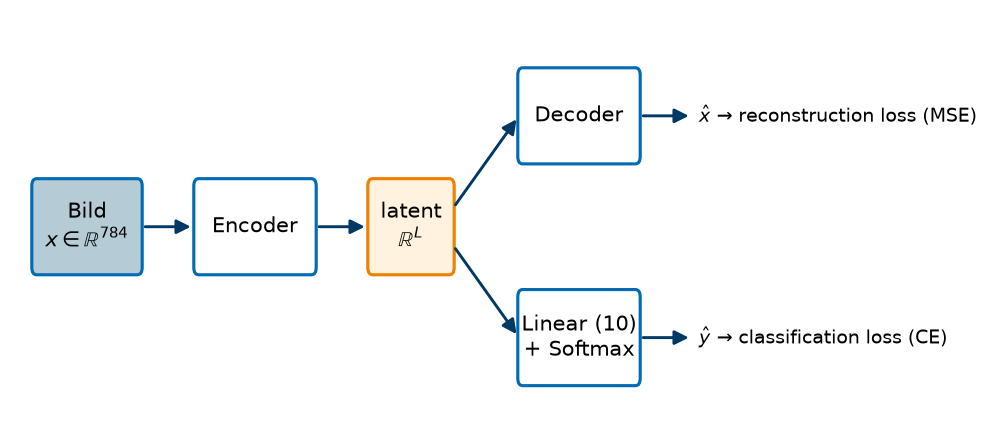
\includegraphics[width=0.62\textwidth]{vl07-label-autoencoder.png}
  \end{center}

  \bigskip
  \begin{center}
    \normalsize $L = \text{reconstruction} + \text{classification}$
  \end{center}

  \note{Ein Encoder, zwei Köpfe, zwei Loss-Terme. Der Encoder muss jetzt einen latenten
    Raum finden, der \emph{beides} kann.
    Die Rekonstruktion wirkt dabei wie eine Regularisierung des Klassifikators --- der
    latente Raum darf nichts Wichtiges wegwerfen. Das ist die Pointe.}
\end{frame}

\begin{frame}
  \frametitle{Tricks bei der Architektur}

  \begin{itemize}\setlength{\itemsep}{8pt}
  \item Mehr Layer
  \item Swish statt ReLU (\texttt{nn.SiLU})
  \item \textbf{Dropout}: zufällig 30\,\% auf null, nur im Training
  \item \textbf{BatchNorm}: pro Batch normieren, Skalierung lernbar
  \end{itemize}

  \note{Dropout verhindert, dass sich das Netz auf einzelne Neuronen verlässt --- wirkt
    gegen Overfitting.
    BatchNorm: Mittelwert abziehen, durch Standardabweichung teilen, beides über den
    Batch. Warum das hilft, ist theoretisch kompliziert; praktisch hilft es. Der
    Zusammenhang zur Feature-Skalierung aus VL 5 ist derselbe Gedanke, eine Schicht tiefer.}
\end{frame}

\begin{frame}
  \frametitle{Sparse Autoencoder}

  \begin{center}
    \Large
    $L_{\text{sparse}} = \sum_j D_{KL}\bigl(\operatorname{Ber}(\varrho)\,\|\,\operatorname{Ber}(\hat\varrho_j)\bigr)$
  \end{center}

  \bigskip
  \begin{center}
    \normalsize mit $\varrho = 0{,}1$: jede Dimension im Mittel zu 10\,\% „an“.
  \end{center}

  \note{Die Loss-Funktion um einen \emph{Strafterm} ergänzen --- das ist das Muster, das
    nächste Woche beim VAE wiederkommt.
    \textbf{Praktischer Hinweis, der Zeit spart:} Der Term muss im Code ausdrücklich
    addiert werden, \texttt{loss = reconstruction\_loss + beta * sparsity\_loss}. Eine
    Funktion, die ihn nur berechnet, ändert am Training gar nichts --- ein Fehler, den
    man einmal macht.}
\end{frame}

\begin{frame}
  \frametitle{Dicht gegen dünn besetzt}

  \begin{center}
    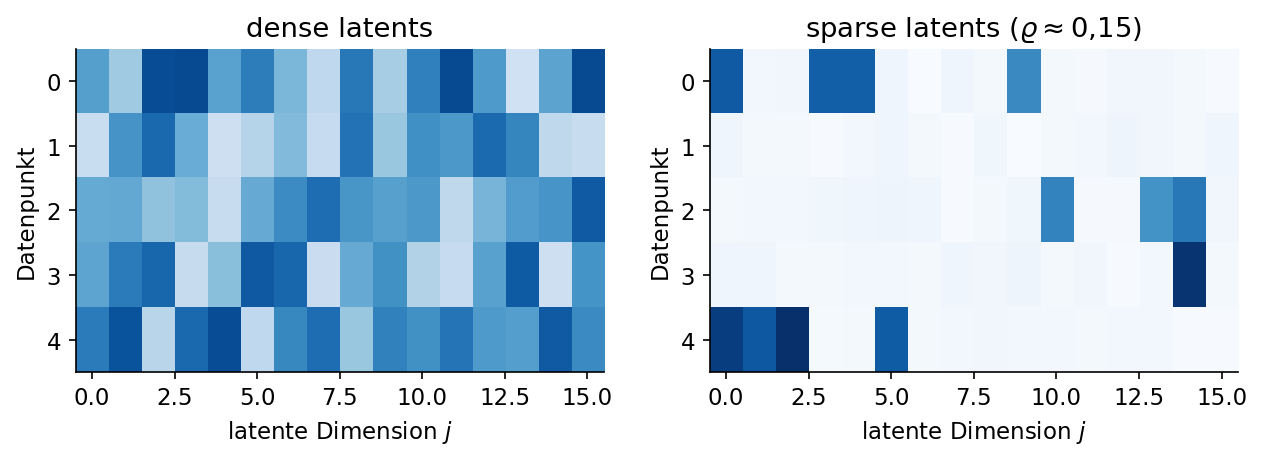
\includegraphics[width=0.72\textwidth]{vl08-sparse-vs-dense.png}
  \end{center}

  \note{Fünf Datenpunkte (Zeilen), 16 latente Dimensionen (Spalten).
    Dense nutzt alle Dimensionen für jeden Punkt; sparse verteilt die Punkte auf wenige
    aktive Dimensionen --- das macht die einzelnen Dimensionen interpretierbarer. Genau
    deshalb sind Sparse Autoencoder gerade in der Interpretierbarkeitsforschung populär.}
\end{frame}

\begin{frame}
  \frametitle{Denoising Autoencoder}

  \begin{center}
    \Large
    Eingabe: $x + \varepsilon$\\[12pt]
    Ziel: das \emph{saubere} $x$
  \end{center}

  \bigskip
  \begin{center}
    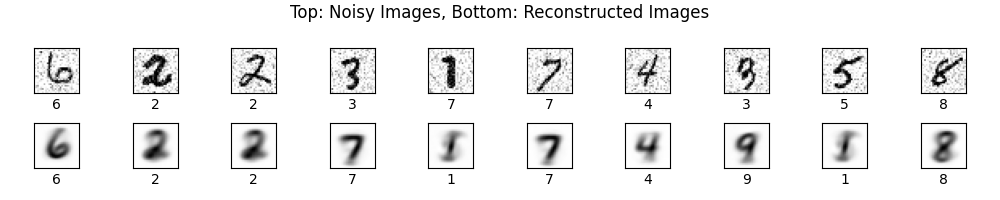
\includegraphics[width=0.5\textwidth]{vl08-denoising-example.png}
  \end{center}

  \note{Daten nicht putzen, sondern verschmutzen --- und das Netz lernt, den Schmutz zu
    entfernen. Der latente Raum muss dann das Wesentliche behalten.
    Das ist dieselbe Idee wie beim Lückentext in BERT (VL 3) und bei word2vec (nächste
    Woche): kaputt machen, wiederherstellen lassen.}
\end{frame}

\begin{frame}
  \frametitle{Blatt 8}

  \begin{center}
    \Large MNIST-Autoencoder selbst bauen.
  \end{center}

  \bigskip
  \begin{center}
    Nächste Woche: den latenten Raum \emph{sampeln} --- VAE und word2vec.
  \end{center}

  \note{Tipp fürs Blatt: erst zum Laufen bringen, dann hübsch machen. Adam nehmen, sonst
    sieht man nichts. Rekonstruktionen plotten, nicht nur den Loss angucken.}
\end{frame}

\end{document}

%%% Local Variables:
%%% mode: latex
%%% TeX-master: t
%%% End:
